\documentclass{mp}
\subtitle{Uwagi organizacyjne}
\begin{document}
\begin{frame}
\titlepage
\end{frame}
\begin{frame}{Kontakt}
mgr inż. Jędrzej Potoniec \\
\url{Jedrzej.Potoniec@cs.put.poznan.pl}\\
\url{http://www.cs.put.poznan.pl/jpotoniec}
\end{frame}
\begin{frame}{Zasady oceniania}
Egzamin zaliczający obie części przedmiotu:
\begin{description}
\item[ćwiczenia] 75\% puntków
\item[wykład] 25\% punktów
\item[można] mieć kartkę ze wzorami i~kalkulator (bez Wi-Fi, GSM itp)
\item[nie można] komunikować się z innymi
\item[nie trzeba] uczyć się na pamięc definicji, twierdzeń (ale trzeba je umieć stosować!)
\item[dodatkowo] punkty za aktywność
\end{description}
\end{frame}
\begin{frame}{Skala ocen}
\begin{center}
\begin{tabular}{l|r}
\% punktów & ocena \\
\hline
$\left(-\infty; 50\right]$ & 2,0 \\
$\left(50; 60\right]$ & 3,0 \\
$\left(60; 70\right]$ & 3,5 \\
$\left(70; 80\right]$ & 4,0 \\
$\left(80; 90\right]$ & 4,5 \\
$\left(90; \infty\right)$ & 5,0 \\
\end{tabular}
\end{center}
\end{frame}
\begin{frame}{Obecność}
\begin{block}{Regulamin studiów, rozdział II, par.8 pkt. 2}
Uczestnictwo w zajęciach objętych planem studiów jest obowiązkowe dla nauczycieli akademickich i~studentów.
Uczestnictwo w ćwiczeniach, zajęciach laboratoryjnych, projektowych, seminariach, pracowniach, lektoratach i~zajęciach WF jest kontrolowane przez prowadzącego.
\end{block}
{\tiny Regulamin studiów uchwalony przez Senat Akademicki Politechniki Poznańskiej Uchwałą Nr 175 z dnia 25 kwietnia 2012 r. Zmiany wprowadzone Uchwałą Nr 185 z dnia 27 czerwca 2012 r.}
\end{frame}
\begin{frame}{Inspiracje}
\begin{itemize}
\item \emph{Metody probabilistyczne} prof. J. Węglarz @ PUT
\item \emph{CS 223 -- Random Processes and Algorithms} @ Harvard \\
\url{http://www.eecs.harvard.edu/~michaelm/CS223/}
\end{itemize}
\end{frame}
\begin{frame}{Literatura}
\begin{itemize}
\only<+>{\item M. Mitzenmacher, E. Upfal \emph{Metody probabilistyczne i~obliczenia} (WNT 2009) \\
	\centering
\includegraphics[height=.7\textheight]{books/met_prob.jpg}
}
\only<+>{\item W. Krysicki, J. Bartos i~in. \emph{Rachunek prawdopodobieństwa i~statystyka matematyczna w zadaniach} (PWN 2010)\\
\centering
\includegraphics[height=.7\textheight]{books/rachunek-prawdopodobiestwa-i-statystyka-matematyczna-w-zadaniach-cz-1_4104.jpg}
}
\only<+>{\item A. Plucińska, E. Pluciński \emph{Probabilistyka: rachunek prawdopodobieństwa, statystyka matematyczna, procesy stochastyczne} (WNT 2000)\\
\centering
\includegraphics[height=.7\textheight]{books/plucinscy.jpg}
}
\only<+>{\item Amir D. Aczel \emph{Statystyka w zarządzaniu} (PWN 2006)\\
\centering
\includegraphics[height=.7\textheight]{books/aczel.jpg}}
\only<+>{\item S. Takahashi, Trend-Pro Co. Ltd. \emph{The Manga Guide to Statistics} (No starch press 2008)\\
\centering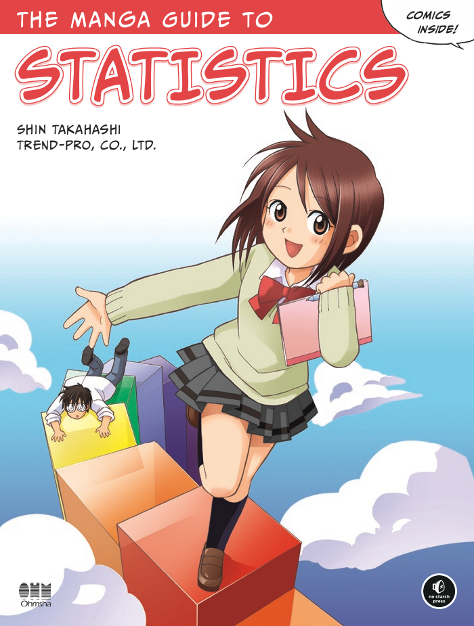
\includegraphics[height=.7\textheight]{books/mg_statistics_big.png}}
\only<+>{\item M. Heller \emph{Filozofia przypadku: kosmiczna fuga z preludium i~coda} (Copernicus Center Press 2012)\\
\centering
\includegraphics[height=.7\textheight]{books/heller.jpg}}
\only<+>{\item Eliezer Yudkowsky \emph{Harry Potter and the Methods of Rationality} \url{http://hpmor.com/}\\
\centering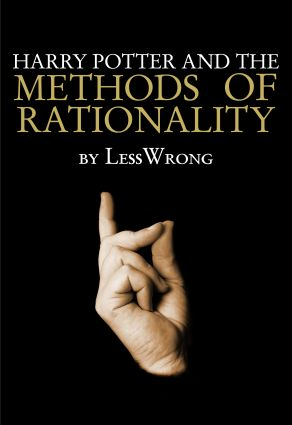
\includegraphics[height=.7\textheight]{books/hpmor.jpg}}
\end{itemize}
\end{frame}
\begin{frame}{Plan wykładu}
\begin{enumerate}
\item Wstęp
\only<+>{\begin{enumerate}
\item Informacje organizacyjne
\item \emph{Zastosowania probabilistyki w informatyce}
\end{enumerate}}
\item Aksjomatyka rachunku prawdopodobieństwa
\only<+>{\begin{enumerate}
\item Przestrzeń zdarzeń elementarnych
\item Zdarzenia i działania na nich
\item Aksjomatyczna definicja prawdopodobieństwa
\item \emph{Probabilistyczne porównywanie wielomianów}
\item Prawdopodobieństwo warunkowe, zupełne i twierdzenie Bayesa
\item Niezależność zdarzeń
\item \emph{Klasyfikator Bayesa i filtry antyspamowe}
\end{enumerate}}
\item Zmienne losowe
\only<+>{
	\begin{enumerate}
	\item Pojęcie zmiennej losowej, funkcji prawdopodobieństwa i~dystrybuanty
	\item Typy zmiennych losowych
	\item Momenty zmiennych losowych, nierówności Markowa i~Czebyszewa
	\item \emph{Podstawowa metoda Monte-Carlo}
	\item Przykładowe rozkłady prawdopodobieństwa: jednostajne, dwupunktowy, dwumianowy, Poissona, geometryczny, Gaussa
	\item Problem znakowania pakietów
	\item Dwuwymiarowe zmienne losowe
	\item Kowariancja, korelacja, regresja
	\item Ciągi zmiennych losowych
	\item Twierdzenia graniczne
	\end{enumerate}
}
\item Procesy losowe
\only<+>{
	\begin{enumerate}
\item Pojęcie procesu losowego i jego opis
\item Momenty procesu losowego
\item Procesy stacjonarne
\item Procesy o przyrostach niezależnych, procesy Markowa
\item Rozkład wykładniczy
\item Proces Poissona
\item \emph{Kolejka \texttt{M|M|1}}
\end{enumerate}}
\end{enumerate}
\end{frame}
\begin{frame}{Harmonogram wykładów}
\begin{description}
\item[28.02] %TODO
\item[09.05]
\item[30.05]
\item[14.06]
\end{description}
\end{frame}
\begin{frame}{Harmonogram ćwiczeń}
\begin{description}
\item[10.05] %TODO
\item[16.05]
\item[30/31.05]
\item[20.06]
\end{description}
\end{frame}

\end{document}
